%\newcommand{\eps}{\epsilon}
\newcommand{\Pmax}{p_\text{max}} 	
\newcommand{\Hint}{H_{int}}
\newcommand{\kbar}{\bar{k}}
\newcommand{\Delk}{\Delta}
\newcommand{\Sumk}{\Sigma}
\newcommand{\Qrot}{Q_{pq}(\tau_s)}
\newcommand{\shapecor}{\mathcal{S}}
\newcommand{\ampcor}{\mathcal{A}}
\newcommand{\totalcor}{\mathcal{E}}
\newcommand{\threeLs}{L_p(\kbar_1)L_q(\kbar_2)L_r(\kbar_3)}
\newcommand{\threePs}{P_p(\kbar_1)P_q(\kbar_2)P_r(\kbar_3)}
\newcommand{\threeQs}{Q_p(k_1)Q_q(k_2)Q_r(k_3)}
\newcommand{\Lbasic}{\mathcal{P}_0}
\newcommand{\Linvk}{\mathcal{P}_1}
\newcommand{\Lnsinv}{\mathcal{P}^{n_s}_1}
\newcommand{\Lnsboth}{\mathcal{P}^{n_s}_{01}}
\newcommand{\Linvksq}{\mathcal{P}_2}
\newcommand{\Lns}{\mathcal{P}^{n_s}_2}
\newcommand{\Fbasic}{\mathcal{F}_0}
\newcommand{\Finvk}{\mathcal{F}_1}
\newcommand{\Finvksq}{\mathcal{F}_2}
\newcommand{\quadpot}{V_{\phi^2}(\phi)}
%\newcommand{\threeqs}{q_p(\kbar_1)\,q_r(\kbar_2)\,q_s(\kbar_3)}
\newcommand{\threeqs}{q_p(k_1)\,q_r(k_2)\,q_s(k_3)}
\newcommand{\threeqstilde}{q_{\tilde{p}}(k_1)\,q_{\tilde{r}}(k_2)\,q_{\tilde{s}}(k_3)}
\newcommand{\kmin}{{k_\text{min}}}
\newcommand{\kmax}{{k_\text{max}}}
\newcommand{\fnl}{f_{NL}}
\newcommand{\fnllocal}{f^{local}_{NL}}
\newcommand{\fnlequil}{f^{equil}_{NL}}
\newcommand{\fnlortho}{f^{ortho}_{NL}}

\chapter{Introduction I: Cosmology}\label{chapter:intro_general}
\section{The standard cosmological history}\label{sec:general_intro}
%\subsection{The bispectrum}
    \subsection{Fundamentals}
\textcolor{red}{Remove some of the plots, sort out ordering. Talk about cosmological constant, curvature?
Blackbody, being able to define a temperature. Define conformal time!
Mention template-free.}


When we look out into the sky, we see light that has traveled for a very long time to get to us.
In that light we see images of the universe as it was when the light left its source.
We see the moon as it was a second ago, or the Andromeda Galaxy as it was millions of
years ago. To what extreme can we push this? How far back in time can we see? As we look further
away, and further back in time, we see a universe that looks nothing like the one we know today.
We see a universe that was extremely hot and dense, but also extremely uniform---whereas today
we have distinct galaxies and the empty spaces in between, looking far enough back we see a universe
without that structure, instead simply uniformly hot and dense everywhere.


But this uniformity wasn't perfect. There were patches that were very slightly more dense than the average,
and others that were very slightly less dense. These non-uniformities provided the seeds that would form
structure---the over-dense regions had a slightly higher gravitational pull on their surroundings,
and caused the nearby matter to begin to fall in. This process would eventually result in the structure
we see in the universe today: the stars, the galaxies, and all the complexity on our own planet.


The precise details of this story have been fleshed out thanks to the work of many people.
It is incredible that we can say so much about the radically different epochs of the universe that came before our own,
between this hot, dense initial state and today.
More work remains to be done, however---one aspect we can question is the origin of the non-uniformities
that provided the seeds of structure. What was the physics that generated them?
The goal of the work described in this thesis is to develop methods to connect this physics
to the sky we see today; more precisely, we aim to use the light from the early universe (the cosmic microwave
background, the $\cmb$)
to constrain physical theories of the very early universe (the epoch of inflation) using a particular
statistical description, known as the bispectrum.
We aim to mature the connection between models of inflation and their predicted bispectra, so we can better
extract the fundamental physics waiting to be found in the universe's youth.


    General relativity is the theory which describes how the evolution of the universe depends
    on its matter and energy content. It describes the path of light as a geodesic, a straight line
    in spacetime---with spacetime being described in terms of curved geometry.
    The equations that we derive from this theory (the Einstein equations) are written in terms of a metric,
    which we denote by $g_{\mu\nu}$. This object defines our notion of distance, and thus encodes
    the causal structure of the universe---which events can influence which other events.
    

    Spatially homogeneous and isotropic universes (i.e.\ ones that at some given
    time, look the same everywhere and in every direction)
    define a class of solutions to the Einstein equations.
    The metric of each universe is known as a Friedmann–Lemaître–Robertson–Walker metric
    (or more usually, and FLRW metric) and in this context
    the Einstein equations become the Friedmann equations, which we will soon present.


    The form of the FLRW metric (we will always set the speed of light to unity\footnote{
        We will also set $\hbar=M_P^{-1}=\sqrt{8\pi G}=1$.
    }) is
    \begin{align}\label{flrw_metric}
        ds^2 = g_{\mu\nu}dx^{\mu}dx^{\nu} = - dt^2 + a(t)^2 dS_3^2
    \end{align}
    where $a(t)$ will have the interpretation as the scale factor
    which describes the evolution of the universe.
    The homogeneity, isotropy and curvature of space are encoded in $dS_3$,
    but a non-trivial time dependence of $a(t)$ breaks the homogeneity of time.
    The components of the matter and energy content of the universe enter the equations through
    their stress-energy tensors, which we approximate as that of
    a perfect fluid (denoted $X$)
    \begin{align}
        T_X^{\mu\nu} = (\rho_X+P_X)U_X^\mu U_X^\nu+P_Xg^{\mu\nu},
    \end{align}
    where the index structure ensures the fluid is isotropic in its rest frame.
    These fluids are completely characterised by the time dependence
    of their energy density $\rho_X(t)$ and their pressure density $P_X(t)$,
    both of which have no dependence on $\vecx$, to preserve the homogeneity of the solution.
    For the components of the universe that we wish to describe,
    taking the quantity $w_X=\frac{P_X}{\rho_X}$ as constant will be a good description.
    This quantity $w$ takes the values $0$, $1/3$ and $-1$ for matter, radiation
    and dark energy (described by a cosmological constant) respectively.
    If we take the spatial curvature of the universe to be vanishingly small,
    the Einstein equation are then
    \begin{align}\label{einstein_equations}
        G_{\mu\nu} = 8\pi G T_{\mu\nu}
    \end{align}
    where $G_{\mu\nu}$ is a complicated function of $g_{\mu\nu}$.
    Fortunately, when $g_{\mu\nu}$ takes the form~\eqref{flrw_metric},
    these equations simplify as promised to the Friedmann equations
    \begin{align}\label{friedmann_1}
        H^2 &= \frac{8\pi G \rho}{3},\\
        \frac{\ddot{a}}{a} &= -\frac{4\pi G}{3}\left(\rho+3P\right),
    \end{align}
    where $H=\frac{\dot{a}}{a}$, and $\rho$ and $P$ are respectively the sum of the
    energy densities and of the pressure densities of the
    components of the universe. We also have the continuity equation
    \begin{align}\label{continuity_equation}
        \dot{\rho}_X + 3\frac{\dot{a}}{a}\left(\rho_X+P_X\right) &= 0
    \end{align}
    which is satisfied for each component separately.

    Given the equations of state and the densities of the different
    components of the universe, one can then calculate the time dependence of the
    scale factor $a(t)$ and of the densities $\rho_X$ and $P_X$ of each component $X$.
    This defines the homogeneous background evolution of the universe---physical phenomena
    such as the redshifting of photons as they freestream through the universe.
    Photons travel on geodesics. The geodesic equation that we use to determine
    their evolution is
    \begin{align}\label{geodesic_eqn_1}
        \frac{dP^\mu}{d\lambda}+\Gamma^\mu_{\nu\sigma}P^\nu P^\sigma=0
    \end{align}
    where $P^a$ is the photon's $4$-momentum, and $\lambda$ is an affine parameter
    for the path.
    The Christoffel symbols, $\Gamma^\mu_{\nu\sigma}$ are functions of the
    metric, and are used to build the $G_{\mu\nu}$ that appeared in the Einstein equations~\eqref{einstein_equations}
    \begin{align}\label{christoffel_symbols}
        \Gamma^\mu_{\nu\sigma} = \frac{1}{2}g^{\mu\gamma}\left(
        \frac{\partial g_{\gamma\nu}}{\partial x^{\sigma}}
        +\frac{\partial g_{\gamma\sigma}}{\partial x^{\nu}}
        -\frac{\partial g_{\nu\sigma}}{\partial x^{\gamma}}
        \right)
    \end{align}
    Using the chain rule,~\eqref{geodesic_eqn_1} can be rewritten in terms of $t$
    \begin{align}
        P^{0}\frac{\partial P^\mu}{\partial t}+\Gamma^\mu_{\nu\sigma}P^\nu P^\sigma=0.
    \end{align}
    Writing the components of the photon's null vector 4-momentum $P^\mu$
    as $(p, \mathbf{p})$, and evaluating~\eqref{christoffel_symbols}
    for the metric~\eqref{flrw_metric} we get that
    \begin{align}
        p\propto \frac{1}{a}.
    \end{align}
    The interpretation of this result is that as the universe expands,
    the photon's measured energy decreases, and its measured wavelength increases.
    The geodesic equation~\eqref{geodesic_eqn_1} encodes many other physical effects when applied
    to the evolution of perturbations around the homogeneous background
    (i.e.\, allowing $g_{\mu\nu}$ to deviate from homogeneity)
    allowing us to understand how the statistics of the perturbations at the
    start of the $\lcdm$ evolution evolved into the perturbations we see today.


    \begin{table}[h!]
    \begin{center}
        \begin{tabular}{ c c c c }
            Epoch & $w$ & $a(t)$ & $a(\tau)$ \\ 
            \toprule
            Radiation & $\frac{1}{3}$ & $t^{\frac{1}{2}}$ & $\tau$ \\
            Matter & $0$ & $t^{\frac{2}{3}}$ & $\tau^2$ \\
            $\Lambda$ & $-1$ & $e^{Ht}$ & $-\frac{1}{\tau}$
        \end{tabular}\caption{
            How the scale factor, $a(t)$, evolves in the
            different epochs of the universe.
        }\label{lcdm_dep_table}
    \end{center}
    \end{table}



    %Since the photon gas has a black body spectrum \textcolor{red}{TALK ABOUT THIS}
    %and is in thermal equilibrium we can assign a temperature to it.
    %This temperature evolves as $T\propto a^{-1}$ away from decoupling temperatures.
    Using~\eqref{continuity_equation} and the equation of state ($w$, summarised in table~\ref{lcdm_dep_table})
    for matter, radiation and dark energy (described as a cosmological constant $\Lambda$)
    we can solve for the dependence of $\rho_X$ on $a$.
    For matter, we obtain the simple result that $\rho_m\propto a^{-3}$,
    i.e.\ that it dilutes with the expansion of the universe.
    For radiation we find $\rho_r\propto a^{-4}$,
    i.e.\ that it dilutes with the expansion of the universe,
    and also loses energy as it redshifts.
    For $\Lambda$, we find $\rho_\Lambda\propto a^0$, by design.
    The Friedmann equation~\eqref{friedmann_1} then gives the time dependence of
    $a(t)$, again summarised in table~\ref{lcdm_dep_table}.


    Using this knowledge we can
    rewrite the Friedmann equation~\eqref{friedmann_1} as
    \begin{align}\label{friedmann_omega}
        H^2 = H_0^2\left(\frac{\Omega_{r,0}}{a^4}+\frac{\Omega_{m,0}}{a^3}+\Omega_{\Lambda}\right)
    \end{align}
    where we define the fractional density
    \begin{align}
        \Omega_{X} = \frac{\rho_X}{\rho_{crit,0}}
    \end{align}
    for $X$ being radiation, matter and dark energy.
    The critical density $\rho_{crit,0}$ is the density for which the universe is flat.


    The measured values for these quantities, as presented in~\cite{Planck_parameters_2018},
    are
    \begin{align}\label{measured_params}
        \Omega_{m,0} &= 0.3111 \pm 0.0056,\\
        \Omega_{\Lambda} &=  0.6889 \pm 0.0056.
    \end{align}
    Since
    $\rho = \frac{\pi^2}{15}T^4$
    for photons, and $T_{\gamma}=2.725\pm0.001K$ \textcolor{red}{CHECK THIS},
    we have that $\rho_{\gamma}=2.02\times 10^{-15} eV^4$
    and $\rho_{crit}=9\times 10^{-27} kg~m^{-3}$.
    Therefore, $\Omega_{\gamma,0}h^2=2.47\times 10^{-5}$.


    From these numbers, and~\eqref{friedmann_omega}, we can make some statements
    about the past and future of the universe, illustrated in figure~\ref{fig:lcdm_components}.
    We can see that while $\Lambda$ is dominant now, the transition from matter domination
    to $\Lambda$ domination happened relatively recently in the history of the universe.
    We can see that this domination will continue as the matter and radiation content of the
    universe dilute and redshift away.
    Running the clock backwards, that is towards $a=0$, we see that the matter and radiation had
    higher energy densities in the early universe. Running the clock back far enough, we see
    that despite $\Omega_{\gamma,0}\ll\Omega_{m,0}$, at one stage it was the
    case that $\Omega_{\gamma}\gg\Omega_{m}$, and the universe was dominated by radiation.
    In that early stage of the universe, the temperature was high enough that the photons
    were tightly coupled to the baryons. The photon pressure supported pressure waves in that
    nearly-homogeneous fluid, and the coupling meant that the baryons were dragged along with those
    waves. Once the temperature and density dropped sufficiently that this was no longer the case,
    the baryons were dropped, and instead began to fall back into the gravitational wells that the dark matter
    had meanwhile been forming. The imprints of those pressure waves is thus seen in the positions
    of galaxies today (in the statistics of their separations) and in the acoustic oscillations of the $\cmb$.


    Before focusing our whole attention on the past, let us briefly
    look toward the future of the universe. Eventually $a$ will be
    sufficiently large that $\Omega_{\Lambda}$
    is the dominant contribution to the energy budget of the universe.
    Then
    \begin{align}
        H^2 &= H_0^2\Omega_{\Lambda}\\
        \implies \dot{a} &= \pm H_0\sqrt{\Omega_{\Lambda}}a
    \end{align}
    from which the initial conditions pick out the exponentially expanding solution,\\
    ${a(t)=a_0e^{H_0\sqrt{\Omega_{\Lambda}}\left(t-t_0\right)}}$. Using the Friedmann equation
    for sufficiently far in the future we can rewrite this as
    \begin{align}
        a(t)=a_0e^{H\left(t-t_0\right)}
    \end{align}
    where $H$ is a constant, having frozen in to a factor $\sqrt{\Omega_{\Lambda}}$ smaller than
    its value today.


    One question we can ask is how far light will travel in the lifetime of the universe.
    Since $ds^2=0$ for a photon, if we define the conformal time $\tau$ such that
    \begin{align}\label{conformal_time_defn}
        \frac{d\tau}{dt} = \frac{1}{a},
    \end{align}
    we find that for the photon, $d\chi=d\tau$.
    This means that on a plot of $\chi$ vs. $\tau$, the path of a photon
    will be a line of slope $1$, even in an expanding universe.
    Integrating, we then find that
    \begin{align}
        \tau(t)=\chi(t)=(Ha_0)^{-1}\left(1-e^{-H(t-t_0)}\right)+\tau_0
    \end{align}
    where as usual a $0$ subscript denotes a quantity evaluated today.
    We see that the comoving distance the photon will travel is finite, even though the physical
    distance (and the time taken, $\int a d\chi$) diverges.
    Integrating~\eqref{friedmann_omega} in the same way that generated figure~\ref{fig:lcdm_tau}
    we find that the points that we see in today's $\cmb$ are a comoving distance of $14.2\Gpc$ away.
    We also find the asymptotic value of $\tau$ to be $19.2\Gpc$, indicating that we will never see the
    light that was emitted from the $\cmb$ at comoving distances greater than this.
    Since $a_0=1$, the present physical distance to these points is equal to the comoving distance,
    but this will increase exponentially in the future.
    %This is the behaviour we would also like in the very early universe, as we will see.

\begin{figure}[!pth]
\centering     %%% not \center
    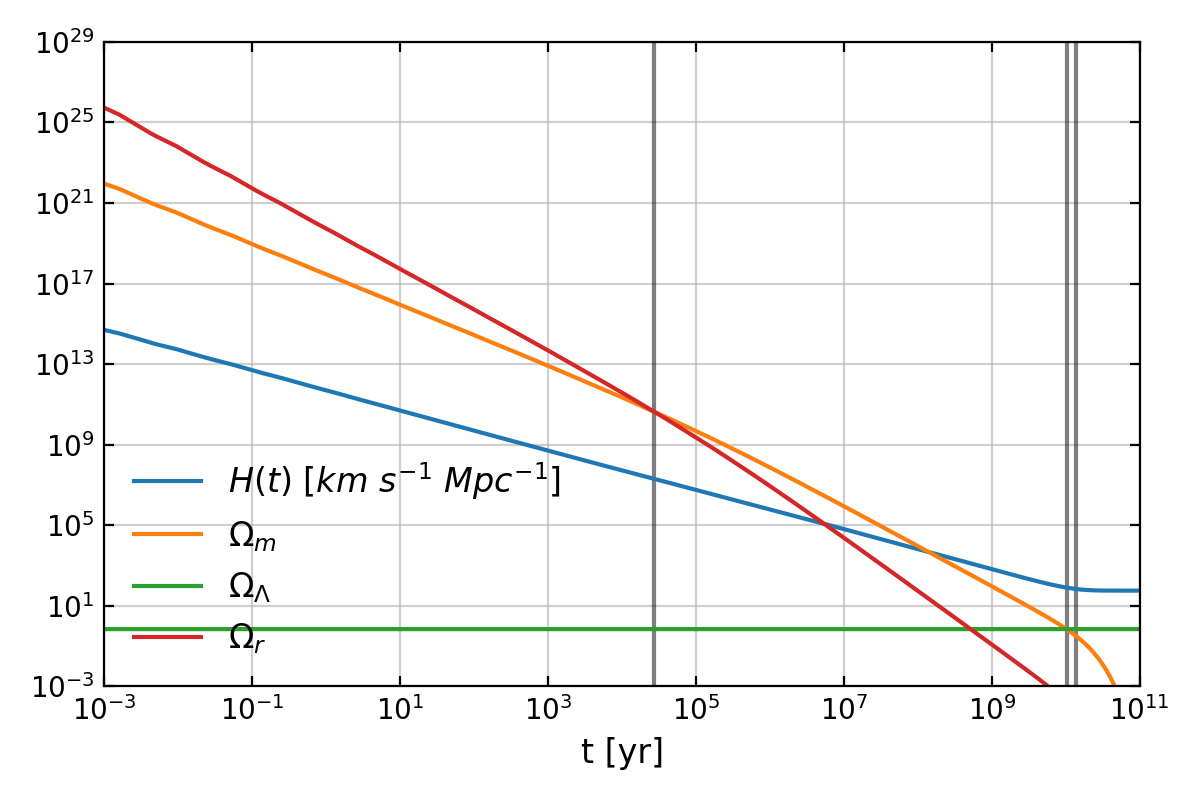
\includegraphics[width=.75\columnwidth]{plots/lcdm_components.png}
\caption{
    The evolution of the components of the universe up to the present, and slightly beyond.
    The vertical grey lines mark matter-radiation equality, matter-dark energy equality,
    and the present day, respectively. We measure these quantities at the present, and
    extrapolate into the past and future using the Friedmann equation~\eqref{friedmann_omega}.
    In the past, densities of matter and radiation were
    far higher, and the radiation energy density dominated over the matter.
    During this high density epoch, the expansion of the universe ($H(t)$) was far stronger.
    In the future, as dark energy comes to dominate, $H(t)$ will become constant.
}\label{fig:lcdm_components}
\end{figure}
\begin{figure}[!pth]
\centering     %%% not \center
    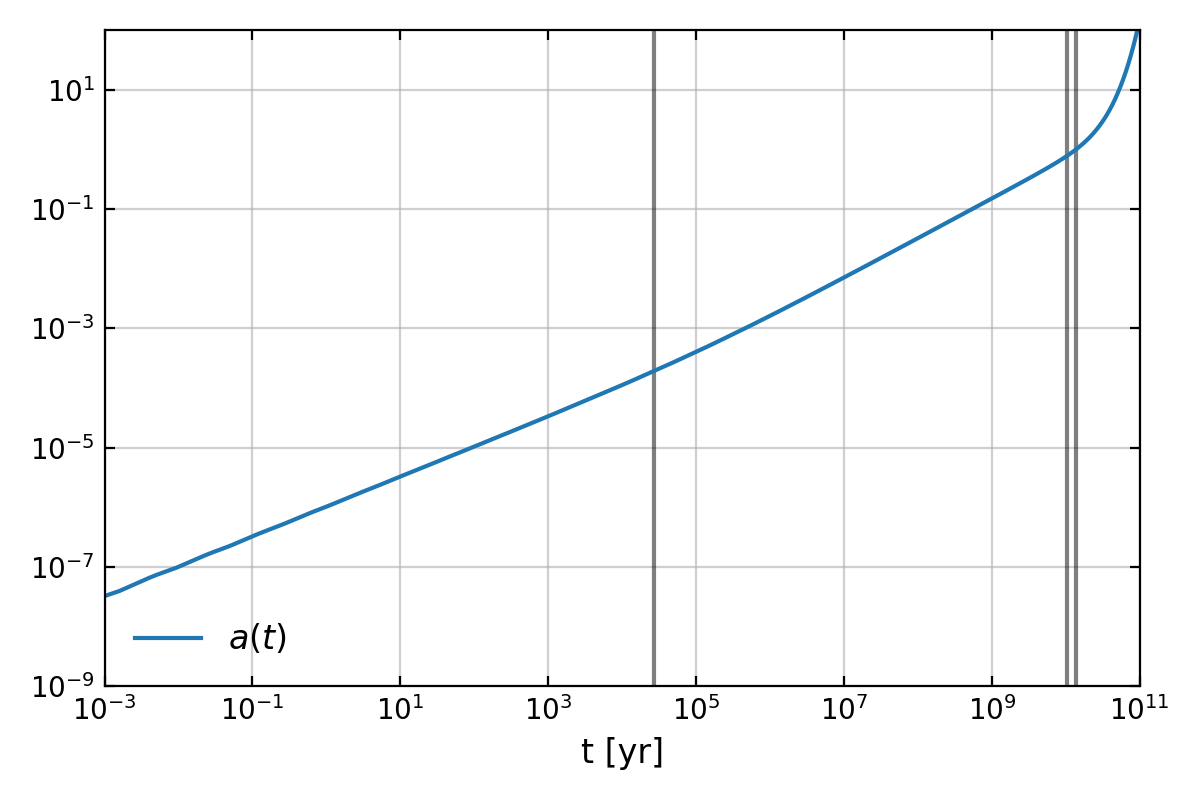
\includegraphics[width=.75\columnwidth]{plots/lcdm_a.png}
\caption{
    The evolution of the scale factor. For most of the $\lcdm$ history
    it evolves as some power of $t$ (see table~\ref{lcdm_dep_table}),
    however as $\Lambda$ comes to dominate
    it will begin to grow exponentially.
}\label{fig:lcdm_a}
\end{figure}
\begin{figure}[!pth]
\centering     %%% not \center
    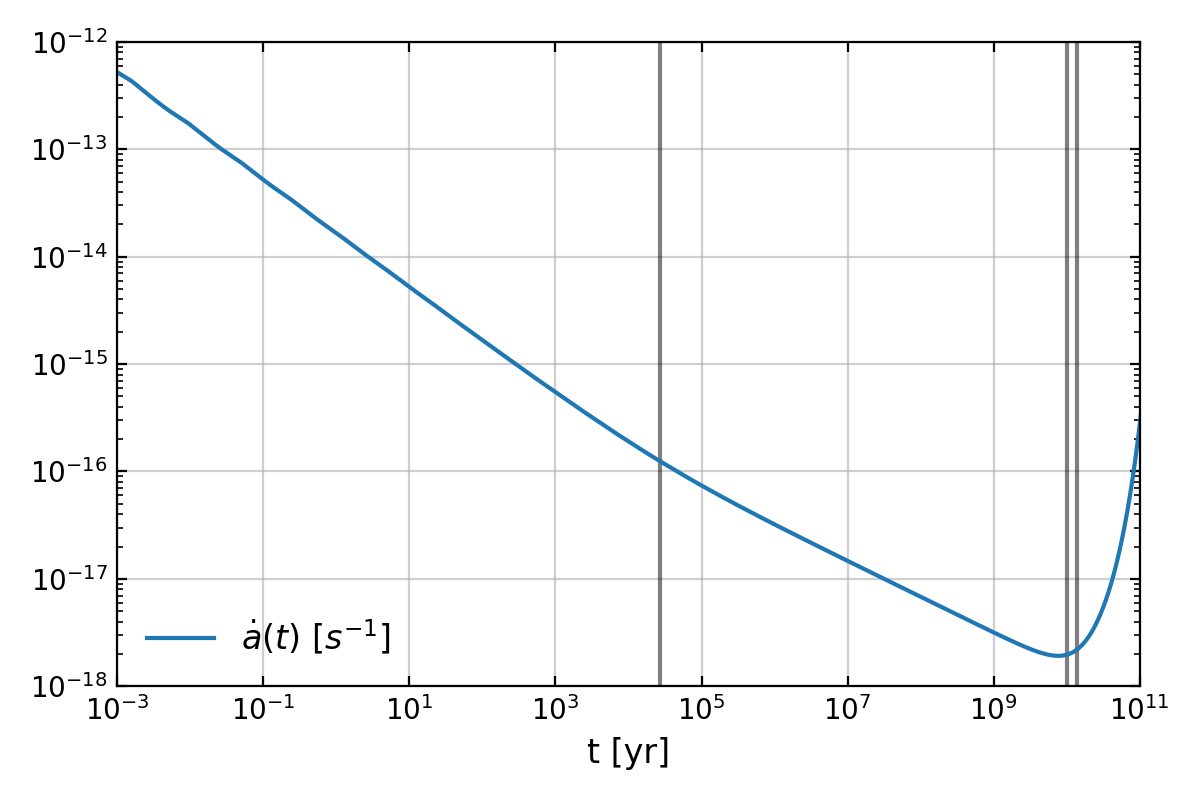
\includegraphics[width=.75\columnwidth]{plots/lcdm_adot.png}
\caption{
    During the radiation and matter dominated eras, the evolution of
    $a(t)$ as been slowing---this is decelerating expansion.
    However, as $\Lambda$ comes to dominate,
    the $\dot{a}$ will begin to increase, and the universe will enter
    and epoch of accelerated expansion.
}\label{fig:lcdm_adot}
\end{figure}
\begin{figure}[!pth]
\centering     %%% not \center
    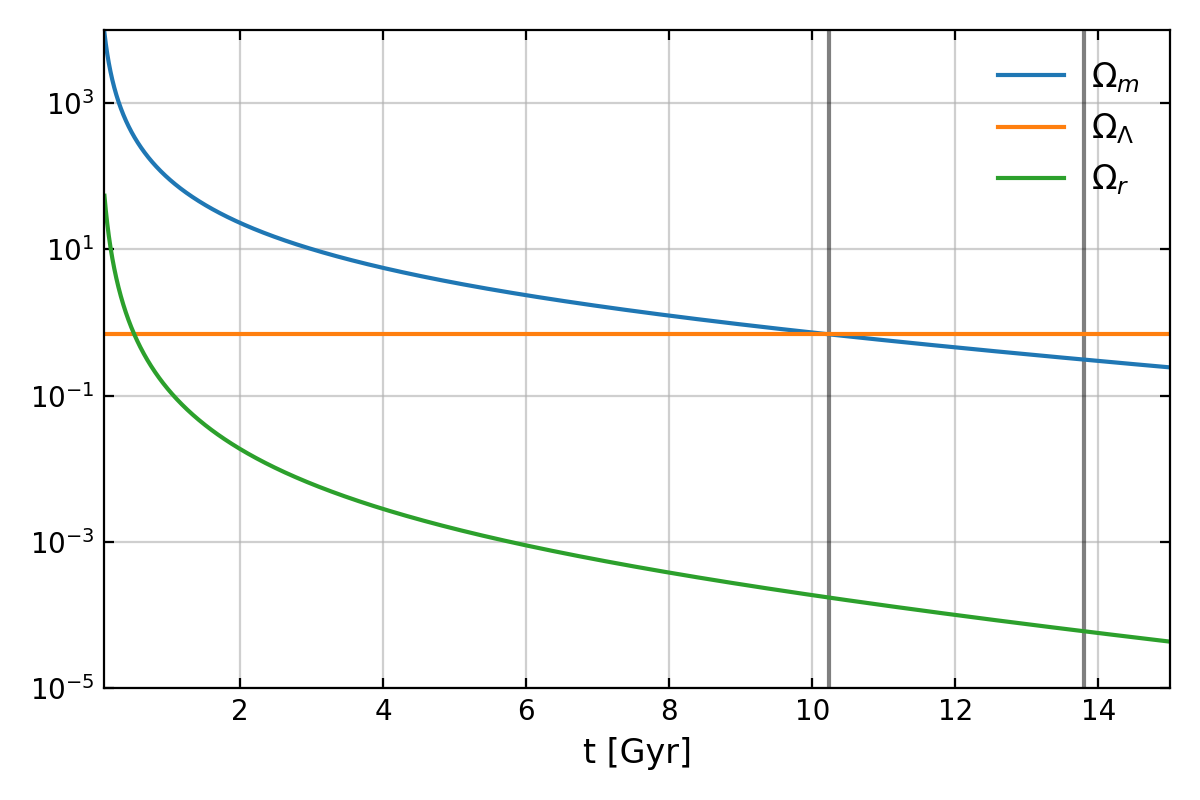
\includegraphics[width=.75\columnwidth]{plots/lcdm_components_linear.png}
\caption{
    The evolution of the components of the universe, zoomed in to more clearly
    show the matter-dark energy transition. The first vertical grey line is
    matter-dark energy equality, the second is the present day.
}\label{fig:lcdm_components_linear}
\end{figure}
\begin{figure}[!pth]
\centering     %%% not \center
    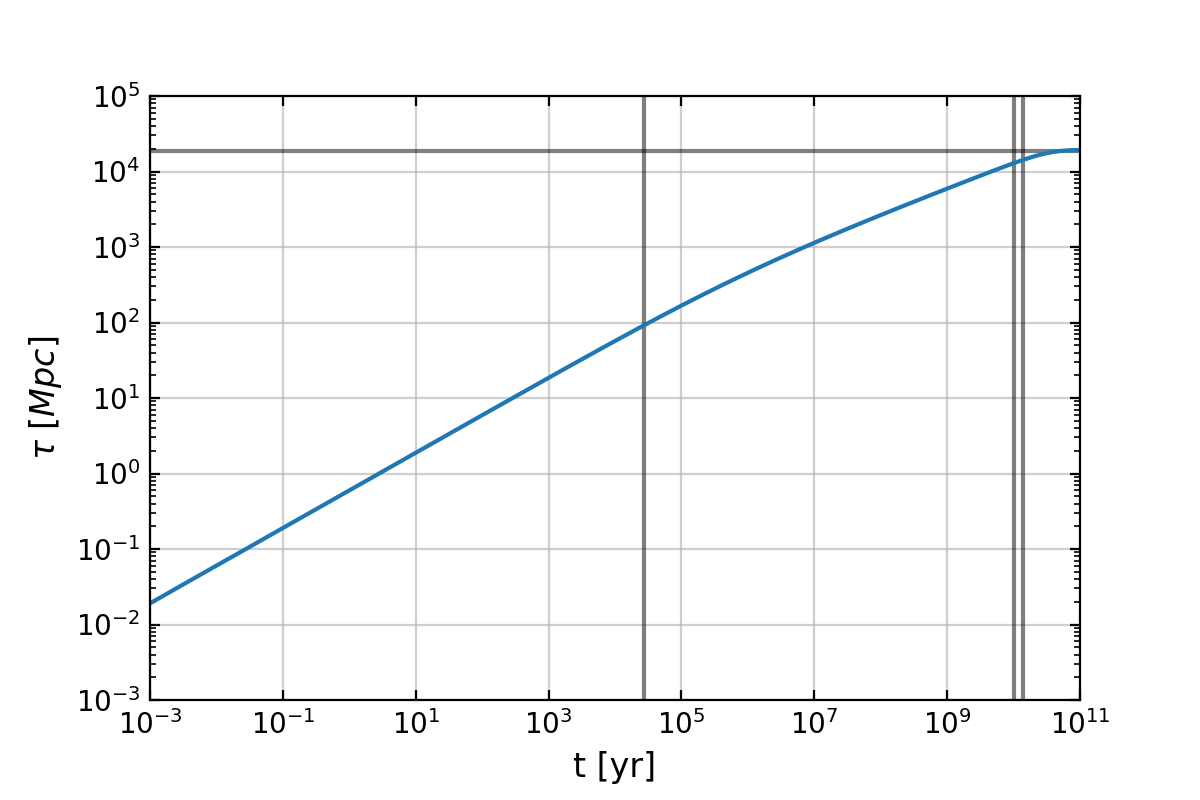
\includegraphics[width=.75\columnwidth]{plots/lcdm_tau.png}
\caption{
    The evolution of the conformal time $\tau$ since the $\lcdm$ singularity,
    if there is no inflation.
    We see that without inflation there is finite conformal time in the past
    \textcolor{red}{do we?},
    and that due to eventual $\Lambda$ dominance
    eventually $\tau$ will asymptote to a constant,
    denoted here by the horizontal grey line at $\tau=\tau_0+(H_0a_0)^{-1}$.
    \textcolor{red}{Physical interpretation at early and late times!!}
}\label{fig:lcdm_tau}
\end{figure}
\begin{figure}[!pth]
\centering     %%% not \center
    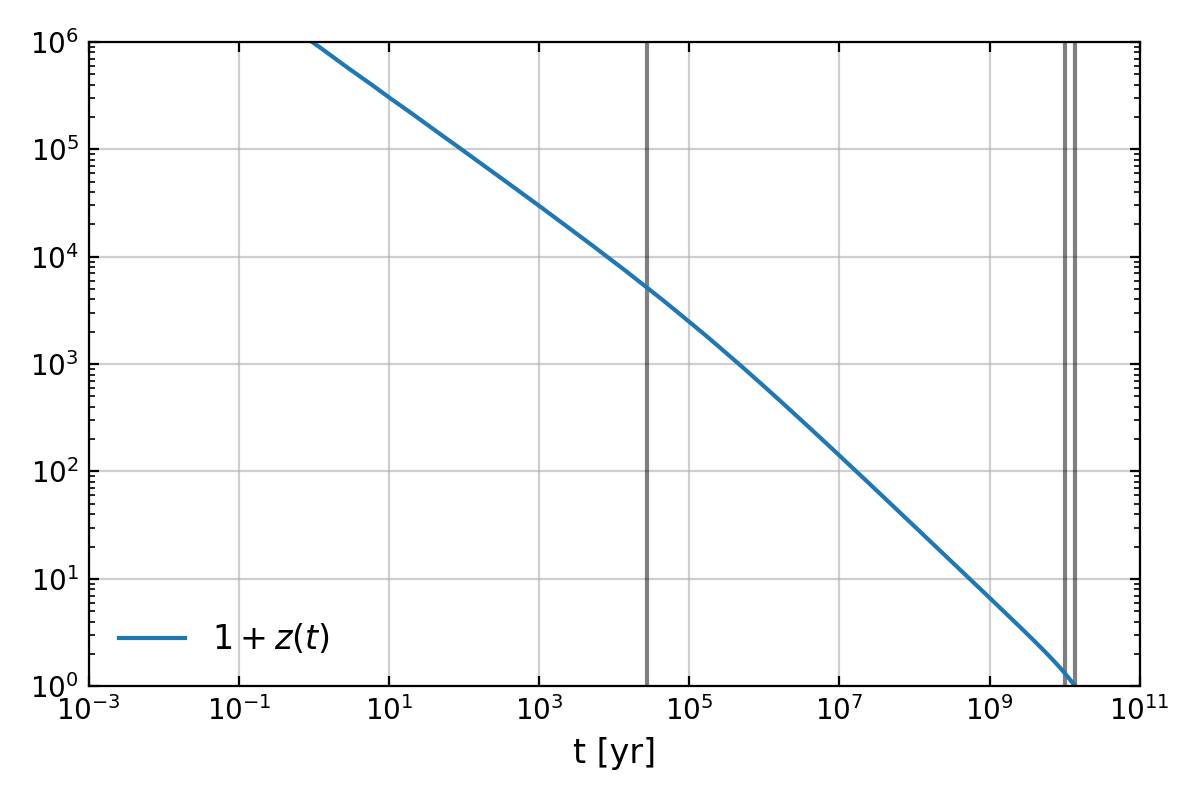
\includegraphics[width=.75\columnwidth]{plots/lcdm_z.png}
\caption{
    The correspondence between redshift $z$ and $t$.
    \textcolor{red}{Talk about the observational effects of having an
    evolving $\dot{a}$, or maybe cut this? Too many plots.}
}\label{fig:lcdm_z}
\end{figure}

    The history of the universe as a story of falling temperature,
    probing higher energy scales. Rough contrast of looking at the
    early universe with particle colliders, cosmic variance etc.
    Maybe mention things like FeynRules or MadGraph?
    \textcolor{red}{Write this, make consistent with elsewhere!}
    \subsection{$\lcdm$}
    \textcolor{red}{Leave this until basically the end, it's least important.
        Add references! Don't explain in detail, but do reference.}
    The $\lcdm$ model of the history of the universe assumes that at some point in the
    past, the components of the universe (all the different types of matter and radiation)
    were in thermal equilibrium with each other---that is, they were interacting with each other,
    and the interaction was sufficiently efficient that their temperatures matched
    and the net flow of thermal energy between them was zero.


    Recombination, what the $\cmb$ is.
    Plot of $a(t)$, $\tau(t)$ over all epochs.
    Path of a photon in $t-x$? Plot of $E(t)$?


    Radiation is one of the major known components of the present universe, in the form of the
    photons in the cosmic microwave background, the $\cmb$. Another is matter, by which we mean \textit{dark} matter,
    which is invisible to our telescopes (which depend on electromagnetic radiation) but can be mapped by the
    effect of its gravity[ref]. Another component is what cosmologists refer to as baryonic matter, which is
    the protons, electrons, neutrons and all the other particles which make up the visible galaxies, stars
    and humans.


    What is the evidence for $\lcdm$? Two main pieces of evidence are the relative abundances of
    primordial elements, and the baryon acoustic oscillations (BAOs).


    While it is thought that the heavier elements are made in incredibly energetic supernovae and
    neutron star collisions (such as lead[ref], or gold[ref]) the lightest elements are instead thought to have been forged in the
    very first minutes of the universes history. The $\lcdm$ model makes a detailed prediction as to the
    relative abundances of these elements, hydrogen, helium and lithium. It works well, but there is
    the ``lithium problem''.


    Baryon acoustic oscillations are the remnants of an epochal transition in the early universe.
    When the baryons decoupled from the radiation (due to the falling temperature) they were dropped,
    no longer supported by the photon pressure. They began to collapse back into the gravitational
    wells the dark matter had been forming. The imprint of this can be seen in the statistics
    of the positions of galaxies in the sky \textcolor{red}{zooming out story} [ref two-point],
    we will discuss two-point statistics in
    section \textcolor{red}{ref}.


    Future work on $\lcdm$ includes the solution of the Hubble tension---how old is the universe really?
    All in all, it is incredible only a hundred years ago people were debating whether the universe had a beginning or not
    (and the ``great debate''---were there other galaxies?) to now, where the debate rages over the second and third significant
    figures.

\section{Initial conditions for $\lcdm$}
    \subsection{Motivations for inflation}
\textcolor{red}{This is important, but shouldn't be long!}
    The $\lcdm$ model does not posit a ``Big Bang singularity'', though this is often
    how it is described in popular science communication.
    \textcolor{red}{Is it a consequence?}
    Instead, as we have discussed, it
    posits an early epoch in which the components that we have discussed are in thermal equilibrium,
    at an incredibly hot temperature of \textcolor{red}{number}. These components are distributed incredibly uniformly,
    with inhomogeneities of less than \textcolor{red}{number}. This simple scenario then evolves
    under gravitational collapse (and other interactions) and forms the universe we know.


    Is this story of $\lcdm$ enough to explain all the features of the
    universe that we observe? The answer is mostly yes, given the correct initial conditions,
    the correct starting point. But then that begs the question of how those initial conditions
    were chosen out of the other possibilities one could imagine.
    Two clues that we have are known as the horizon problem, and the flatness problem.
    Roughly speaking, these problems are the statements that the universe is more homogeneous on
    large scales than we would expect, given the history of $\lcdm$. Why is the temperature on one
    part of the sky so close to the temperature on the other side of the sky? Why is the universe
    so flat?


    To fit observations, $\lcdm$ requires initial conditions with a particular set of properties.
    Some of these properties are surprising, and require an explanation.
    Since $a(\tau)\propto \tau$ during the radiation dominated era we can calculate
    the total comoving distance a photon could have traveled between the singularity at $a_i=0$
    and recombination at $a_{rec}=1/1100$. We find
    \begin{align}
        \chi_{rec} = \int_{0}^{\tau_{rec}} d \tau = \int_{0}^{a_{rec}} \frac{d\tau}{da}da \propto a_{rec}.
    \end{align}
    We can see that this is finite.
    Including the prefactor we find more precisely that $\chi_{rec}=280\Mpc$.
    We can also calculate that the comoving distance that a photon could have
    freely streamed through the universe since
    last scattering is $\chi_0=14000\Mpc$.
    This means that we would expect the homogeneous patches at recombination to span
    at most an angle of
    \begin{align}
        \tan^{-1}\left(2\frac{\chi_{rec}-0}{\chi_{0}-\chi_{rec}}\right) \approx 2^{\circ}
    \end{align}
    on the $\cmb$ sky today. We can then calculate the number of disconnected patches
    we should see as
    \begin{align}
        \frac{4\pi(\chi_{0}-\chi_{rec})^2}{\pi(\chi_{rec}-0)^2} \approx 10^5.
    \end{align}
    This is completely at odds with observations---the $\cmb$ is in fact very close to
    homogeneous \textit{across the entire sky}, clearly a feature of our universe
    that requires an explanation.


    %Photons travelling on $45'$ lines on a $\tau-x$ plot.
    There not being enough time for opposite
    sides of the $\cmb$ to come into thermal equilibrium. But if you change the relation between
    $t$ and $\tau$ then you extend the plot, and you do make contact.
    \textcolor{red}{PLOT THIS? Everyone plots this\ldots}


    The flatness problem is the statement that our universe is much flatter that one would expect.
    The reason we would expect otherwise, is that deviations from flatness are unstable.
    This means that if the universe is very close to flat now (as we measure it to be)
    then it must have been surprisingly close to flat at the beginning of the $\lcdm$
    evolution. A natural explanation of this would be an attractive quality in a
    theory of the very early universe.


    We will mention three more features of the $\lcdm$ initial conditions that we would
    like an explanation for. Those three features are the adiabaticity of the initial
    perturbations, the (as measured so far) Gaussianity of those perturbations, and finally
    the very slight deviation from perfect scale invariance that observations demand the
    initial power spectrum must have had.


    Adiabaticity is the statement that for each of the components of the universe, their
    initial conditions $\delta\rho_i$ were related such that
    \begin{align}
        \frac{\delta\rho_i}{\bar{\rho}'_i} = \frac{\delta\rho_j}{\bar{\rho}'_j}.
    \end{align}
    To phrase this another way, by performing a local reparametrisation of time $t\rightarrow t+\delta t(x)$
    \begin{align}
        \bar{\rho}_i(t)+\delta \rho_i(t,x) = \bar{\rho}_i(t)+\delta t(x)\bar{\rho}'_i
        = \bar{\rho}_i(t+\delta t(x))
    \end{align}
    we can absorb the perturbations in \textit{all} of the components. The implication that we can draw
    is that the initial conditions of these separate components were generated by a process that was simpler than
    it could have been.
\textcolor{red}{But entropy perturbations source adiabatic, right? So how surprising is it really?}


    The Gaussianity of the initial conditions is the statement that their statistics are completely described by
    their two-point function. We will discuss this in more detail in a later section.
    The deviation from perfect scale invariance has been measured to high confidence by the $\planck$
    satellite. \textcolor{red}{Refer to WMAP!}~\cite{Senatore_wmap_2009}.
    Later in section~\ref{corr_functions} we will define scale invariance.
    It turns out that observations show that this is not precisely respected.
    In fact, it was found that $P(k)\propto k^{n_s-4}$, with $n_s=0.9649 \pm 0.0042$.

    \subsection{Driving inflation with a scalar field}
We will work with an inflaton action of the form
\begin{align}
S = \int d^4x \sqrt{-g}P(X,\phi)
\end{align}
with $X=-\frac{1}{2}g^{ab}\nabla_a \phi\nabla_b \phi$.
We work with the number of e-folds, $N$, as our time variable
$x'=\frac{dx}{dN}=a\frac{dx}{da}$
and recall the definitions of the slow-roll parameters~\eqref{slowrollparams},
though we make no assumption that these are actually small.
$c_s$ is the sound speed of the theory, which can vary with time:
\begin{align}
c_s=\frac{P,_X}{P,_X+2XP,_{XX}}.
\end{align}
The background quantities are evolved according to the Friedmann equations,
which are set with consistent initial conditions.
The expression for the energy density is~\cite{Christopherson_2009}
\textcolor{red}{CHECK REFERENCE, REORDER WHOLE SECTION.}
\begin{align}
    \rho = 2XP,_X-P,
\end{align}
so then
\begin{align}
    \rho' = -6XP,_X.
\end{align}


    We take $X=\frac{1}{2}\left(\frac{\partial\phi}{\partial t}\right)^2$.
    The sound speed for the adiabatic perturbation is defined as
    \begin{align}\label{sound_speed_definition}
        c_s^2 = \left. \frac{\partial P}{\partial \rho} \right|_S = \frac{\dot{P}_0}{\dot{\rho}_0}
        = \frac{P,_X}{\rho,_X}.
    \end{align}
    Since we also have $\rho=2X P_X-P$, we see that
    \begin{align}
        c_s^2 = \frac{P,_X}{P_X+2X P_{XX}}.
    \end{align}
    For canonical inflation models, $P(X,\phi)=X-V(\phi)$
    so $P_{XX}=0$ and $c_s=1$.


Then, using the Friedmann equation we obtain
\begin{align}\label{PXepsilon}
    \varepsilon &= -\frac{1}{2}{\phi'}^2P,_X.
\end{align}
The equation of motion for $\phi$ is~\cite{Hu_2011}
\begin{align}\label{phieom}
    \phi''+(3c_s^2-\varepsilon)\phi'+H^{-2}\frac{\rho_\phi}{\rho_X}=0.
\end{align}


    For reasons we will discuss in section~\ref{pert_evol} we will
    define a quantity $\tau_s$
    in analogy with the usual $\tau$ defined in~\eqref{conformal_time_defn}:
    \begin{align}\label{tausdef}
        \tau_s'&=\frac{c_s}{aH},\\
    \end{align}


    We desire a period of exponential expansion in the early universe to explain the
    scale-invariance of the initial perturbations.
    One simple way one could imagine driving this expansion is through a single
    scalar field. This scalar field would have
    \begin{align}
        \rho_\phi &= \frac{1}{2}\dot{\phi}^2+V(\phi)\\
        P_\phi &= \frac{1}{2}\dot{\phi}^2-V(\phi).
    \end{align}
    For successful inflation with a cosmological constant, we want $w=-1$,
    i.e.\ that $V(\phi)\gg\frac{1}{2}\dot{\phi}^2$. Since the kinetic term is required to
    be small, this is referred to as \textit{slow-roll} inflation.
    The Friedmann equations then become
    \begin{align}
        H^2 &\approx \frac{8\pi G}{3}V(\phi),\\
        \frac{\ddot{a}}{a} &\approx -\frac{4\pi G}{3}\left(-2V(\phi)\right).
    \end{align}
We define the Hubble parameter and the standard ``slow-roll'' parameters:
\begin{equation}
\label{slowrollparams}
\begin{split}
    H = \frac{d\ln a}{dt}	\,,
    \qquad
    \eps &= -\frac{d\ln H}{dN}	\\
    \eta = \frac{d\ln \varepsilon}{dN}	\,,
    \qquad
    \eps_s &= +\frac{d\ln c_s}{dN}	\,.
\end{split}
\end{equation}

From the continuity equation and the Friedmann equation
\begin{align}
    &&\rho' &= -3(\rho+P)\\
    \implies&&6HH' &= -3(2X P,_{X})\\
    \implies&&-H^2\varepsilon &= -\left(\frac{1}{2}H^2{\phi'}^2\right) P,_{X}\\
    \implies&&\varepsilon &= \frac{1}{2}{\phi'}^2 P,_{X}.
\end{align}
In the canonical case this simplifies to
$\varepsilon = \frac{1}{2}{\phi'}^2$.
In the DBI case we find
$\varepsilon = \frac{1}{2}\frac{{\phi'}^2}{c_s}$.

This allows us to rephrase the Friedmann equation in the following useful
way. Note that this is still exact, the slow-roll approximation has
not been used.
\begin{align}
    &&H^2 &= \frac{1}{3}\left(\frac{\varepsilon H^2}{P,_{X}}+V(\phi)\right)\\
    \implies &&  H^2 &= \frac{V(\phi)}{3-\frac{\varepsilon}{P,_{X}}}.
\end{align}

\newpage
    \subsection{Criteria for successful inflation}
    \textcolor{red}{Rewrite entirely in terms of $a$, $H$? And move earlier.}
    For inflation to solve the horizon problem, it must result in a shrinking comoving
    Hubble radius, disconnecting regions that had previously been in thermal contact.
    This implies that
    \begin{align}
        \frac{d}{dt}\left(aH\right)^{-1} = -\frac{\ddot{a}}{\dot{a}^2} < 0
    \end{align}
    so $\ddot{a}>0$, i.e.\ the expansion is accelerating. Another way of writing this is
    \begin{align}
        \frac{d}{dt}\left(aH\right)^{-1} &= -\frac{1}{(aH)^2}\left(\dot{a}H+a\dot{H}\right)\\
            &= -\frac{1}{a}\left(1-\varepsilon\right)
    \end{align}
    and so we need $\varepsilon<1$ to successfully inflate the universe.
    This is necessary but not sufficient---we still need to generate
    the correct statistics for the primordial perturbations.
    This implies we must be close to a perfect de Sitter phase, i.e.\ $\varepsilon\ll1$.
    To match the measured deviation from scale-invariance in standard slow-roll
    inflation we would need $\varepsilon\sim O(10^{-2})$.


For a model with a canonical kinetic term,~\eqref{phieom} simplifies
to
\begin{align}
    \phi''+(3-\varepsilon)\phi'+H^{-2}V'(\phi)=0.
\end{align}
In the slow-roll approximation we take assume $\phi''\ll\phi'$,
and so
\begin{align}
    \phi'\approx\frac{V'(\phi)}{3H^2}\approx\frac{V'(\phi)}{V(\phi)}.
\end{align}
From this, we see that demanding that $\varepsilon$ be small places a constraint
on the flatness of the potential in a canonical model.


We also require $\eta\ll1$ to maintain inflation for the sufficient number
of e-folds.


\newpage
\section{Statistical observables}
    \subsection{Checking if dice are fair}
\textcolor{red}{Move earlier.}
    Everything we have discussed until this point has dealt with quantities
    with definite values, that have a definite evolution. This will no longer
    be true when we discuss quantities that have a quantum origin, as
    the prediction of a fundamental quantum theory is a statistical one.
    The true prediction is of a distribution from which our observation will be drawn;
    as such, to link the sky we see to some fundamental theory,
    we must talk in terms of probabilities.


    Our result will be a constraint on an inflationary parameter, stated at e.g.\ $95\%$ confidence.
    For example, if we flipped one fair coin $100$ times, we would expect an even split of heads
    and tails. Should we be suspicious of the fairness of the coin if we instead get $60$ heads
    and $40$ tails? Or $80$ heads and $20$ tails? An event at least as extreme at a $60$-$40$ split
    will occur $3.5\%$ of the time. For a $80$-$20$ split however, the probability of an event that
    extreme is around one part in $10^{10}$, effectively impossible. This means that if we observed
    a trial where a coin came up heads in $80$ out of $100$ cases, we could suspect that out hypothesis
    of fairness was incorrect.
    One can calculate that, for a fair coin, $95\%$ of the time the number of heads will take a value
    between $41$ and $59$. We call this the $95\%$ confidence interval.
    What we wish to do is the opposite, however. Instead of calculating using known probabilities,
    we wish to take a series of observations of some random variable and use these observations
    to estimate the probability distribution that they were drawn from. Given an infinite number
    of observations this task has a straightforward solution, simply plotting the normalised
    histogram of the results. However, in the context of cosmology we will only have a finite amount
    of information available to us, and thus a limit to how well we can ever measure the relevant
    probability distributions. This limitation is known as cosmic variance.



    We quantify this expected scatter around the mean using a quantity known as the standard deviation.
    The standard deviation of a random variable $X$ is the square root of the expected value of the
    squared deviation from the mean $\mu$,
    \begin{align}
        \sigma = \sqrt{E\left[{(X-\mu)}^2\right]}.
    \end{align}
    In our example above of flipping one coin $100$ times, the total number of heads has $\mu=50$
    and $\sigma=5$.

    
    We have only one universe that we can observe, only one draw from the probability distribution
    we are trying to probe. However, there is a lot of information in that one draw.
    \textcolor{red}{Motivate and explain this all better!} This is related to the concept
    of ergodicity. This is the statement that $\left<\cdot\right>$ as an expectation over ensembles
    at a fixed point is the same as the expectation over points for a fixed ensemble.
    This assumes homogeneity, stationarity, and that distant points are uncorrelated.
    In terms of our coin example, this is related to the statement that flipping one coin
    $100$ times should probe the probability distribution in the same way as flipping
    $100$ identical coins once each.
    %Ergodicity: ``In an ergodic scenario, the average outcome of the group is the same as the average outcome of the individual over time. An example of an ergodic systems would be the outcomes of a coin toss (heads/tails). If 100 people flip a coin once or 1 person flips a coin 100 times, you get the same outcome.'' from https://taylorpearson.me/ergodicity/
    % See also https://nms.kcl.ac.uk/eugene.lim/AdvCos/lecture2.pdf


    We can define the expectation value of a function of a discrete or
    continuous random variable $x$, or a functional $F$ of a field configuration $f(x)$, respectively as
    \begin{align}
        \left<f(x)\right> &= \sum_i x_i P(x_i)\label{expectation_value_discrete}\\
        \left<f(x)\right> &= \int dx~x \rho(x)\label{expectation_value_cont}\\
        \left<F\left[f(x)\right]\right> &= \int \mathcal{D}f~F\left[f(x)\right] P\left[f(x)\right]\label{expectation_value_field}
    \end{align}
    where the sum and integral over $x$ are over the values that $x$ can take,
    and the functional integral over $f$ is over all the field configurations
    that $f(x)$ can take.


    In our example of the $100$ coin flips, we used~\eqref{expectation_value_discrete}
    to calculate the mean and standard deviation. For a continuous variable,
    like the average height of a population or the average temperature in a given room,
    we would use~\eqref{expectation_value_cont}. In this thesis, we will be working with
    the expectation value of field configurations, so we will use~\eqref{expectation_value_field}.
    \textcolor{red}{Talk about quantum to classical transition!}
    \begin{align}
        \left<\hat{v}_{\bk}\hat{v}_{\bk'}\right>
                         &= \left<0|\hat{v}_{\bk}\hat{v}_{\bk'}|0\right>\\
                         &= |v_k|^2\left<0\left|\left[\hat{a}_\bk,\hat{a}_{-\bk}^{\dagger}\right]\right|0\right>\\
                         &= |v_k|^2\delta(\bk+\bk')\\
                         &= P_{v}(k)\delta(\bk+\bk')
    \end{align}


    \subsection{Correlation functions}\label{corr_functions}
    \textcolor{red}{If you find yourself in a universe with\ldots}


    Cite~\cite{Planck_inflation_2015, Planck_inflation_2018}.
    The power spectrum and other correlations
    are predicted by inflation. 
    Define n-point correlations, their Fourier transforms, talk about them as observables.
    

    A model of inflation will predict the statistical properties of the distribution of matter
    that forms the initial conditions for the $\lcdm$ evolution of our universe.
    From this, we can calculate the statistical properties of the $\cmb$ sky that we see.
    One such property is the two-point correlation of the temperature $\phi$
    at a point $x$ in space, $\left<\phi(x)\phi(x')\right>$. When there is a large
    separation between $x$ and $x'$ \textcolor{red}{talk about cosmic variance
    of different modes. Angular?}

    Scale invariance is the statement that
    \begin{align}
        \left<f(\mathbf{x})f(\mathbf{x'})\right> = \left<f(\lambda\mathbf{x})f(\lambda\mathbf{x'})\right>.
    \end{align}
    From this, we can see that scale invariance needs $P(k)\propto k^{-3}$.


    The ensemble average~\eqref{expectation_value_field} of a product of two fields is known as the
    two-point correlator, or the two-point function $\left<f(\mathbf{x})f(\mathbf{x'})\right>$.
    There are two properties we wish to immediately impose on this function, and higher order correlators
    (products of more fields). Those conditions are statistical homogeneity and statistical isotropy.
    That is, we demand that the correlators are invariant under translations and rotations---that is,
    while some realisation of the ensemble might have special points (e.g.\ a maximum value),
    when averaged over the entire ensemble these special points are equally likely to appear anywhere in
    the space.


    These conditions on $f(\vecx)$ place useful constraints on the correlators of the
    Fourier transform, $f(\veck)$. They demand the form
    \begin{align}
        \left<f(\mathbf{k_1})f(\mathbf{k_2})\right> &= (2\pi)^3\delta^{(3)}(\mathbf{k_1}+\mathbf{k_2})P(k_1),\\
        \left<f(\mathbf{k_1})f(\mathbf{k_2})f(\mathbf{k_3})\right> &= (2\pi)^3\delta^{(3)}(\mathbf{k_1}+\mathbf{k_2}+\mathbf{k_3})B(k_1,k_2,k_3),
    \end{align}
    where the delta functions come from statistical homogeneity, and the fact that $P(k)$ (the power spectrum)
    and $B(k_1,k_2,k_3)$ depend only on the magnitudes of the vectors ($k=\left|\veck\right|$) is a result
    of demanding statistical isotropy. Note that $\left<f(\mathbf{k_1})f(\mathbf{k_2})f(\mathbf{k_3})\right>$
    has $9$ degrees of freedom, but $B(k_1,k_2,k_3)$ has only three. This is due to the delta function in
    demanding the $\mathbf{k_i}$ sum to a triangle, and since the orientation of this triangle cannot matter,
    three parameters will suffice---we choose the magnitudes.


    We will want to measure these correlations. How can we do that with only access to one realisation
    of the distribution? It is useful to think about the ergodic theorem. Since an integral over
    space can be identified with the ensemble average, we can measure, say, the average temperature
    across space, which should give us an estimate for the average temperature of the ensemble
    (the quantity that will actually be predicted from theory).
    \textcolor{red}{Is this related to large cosmic variance at large scales? See pg 94 of Lyth and Liddle.}


\section{Thesis outline}
    We are now in a position to give a more precise description of the goals, methods
    and results outlined in this thesis.
    Our main goal was to develop an efficient numerical pipeline for
    connecting inflation models directly to observations through the $\cmb$ bispectrum.
    The concrete results we aimed for were constraints on the parameters of inflation models,
    not constraints on phenomenological templates or summary $f_{NL}$ parameters.
    We aimed to obtain the full bispectrum shape information from an inflation scenario,
    not point samples or a limit. The novelty of our goals comes from the separable
    and numerical methods
    granting access to more accurate, and in some cases new, bispectrum shapes.


    To achieve these goals we have developed methods to preserve the
    separability that is built in to the tree-level in-in formalism.
    This will link to a $\cmb$ calculation that will be presented in~\cite{Sohn_2021}.
    That calculation is expensive, but need only be done once per primordial basis.
    This motivates the desire for a basis that converges quickly for a broad range of inflation models,
    and as such we have developed methods to achieve this.


    Our main result is the first development of a formalism
    for calculating the separable expansion we describe to sufficiently
    high orders as to describe inflationary features.
    These methods are implemented in the $\primodal$ code.
    Another result is the recognition and description of the central issue of the
    convergence of the expansion, and in particular how it is affected by the non-physical $k$-configurations.
    The result of our work in circumventing this problem is the development of multiple
    sets of basis functions, which efficiently capture a broad range of bispectra.
    This allowed the first validation of our separable methods on features.
    We also note that
    as a side-effect of this desire for a separable primordial bispectrum,
    the primordial calculation of the inflationary bispectrum that we present is much more efficient
    than previous methods,
    in the sense converges far faster in modes than previous methods would in point samples.


    Our final highlighted result, which we obtained in collaboration, is the connection
    of our inflationary scenario to the $\cmb$ through the $\cmbbest$ code developed
    by Wuhyun Sohn. This allowed us to obtain constraint on the sound speed of DBI
    inflation, $c_s$.


The thesis is organised as follows. In chapter~\ref{chapter:intro_bispectra} we present brief reviews
of the various parts of the pipeline that connects inflation scenarios to observations
through the bispectrum.
We review the usual paradigm of bispectrum estimation in the CMB,
and the motivation for separable bispectra. We review the in-in formalism,
for calculating the tree level bispectrum for a given model of inflation.
We review $P(X,\phi)$ models of inflation as an example, and
some of the usual approximate bispectrum templates
that we aim to bypass.
We will draw our validation scenarios from these models.
We discuss previous numerical codes for
calculating the primordial bispectrum $k$-configuration by $k$-configuration,
which contrasts our separable basis expansion.
We review the previous work in achieving separability through modal expansions
in~\cite{Funakoshi},
and we discuss methods of testing
numerical bispectrum results, defining our relative difference measurement.


We begin chapter~\ref{chapter:decomp} by recasting the usual in-in calculation into an explicitly separable form,
in terms of an expansion in an arbitrary basis.
Since the paradigm we aim to present is only viable if we can find a basis
that can efficiently represent a wide variety of bispectra,
we devote the rest of chapter~\ref{chapter:decomp} to presenting this discussion, which is
distinct and separate from our numerical methods but nonetheless vital.
We discuss the effects of the
non-physical $k$-configurations on the convergence of our expansion on
the tetrapyd, and present multiple efficient basis sets.
In chapter~\ref{chapter:methods} we present the precise methods involved in the
separable formalism and its numerical implementation,
and detail our methods for carefully calculating the coefficients to high order.
In particular in section~\ref{sec:validation} we validate our methods and implementation
on inflation scenarios with varied features from the literature.
We present a constraint on an inflation model in chapter~\ref{chapter:constraints},
and finish with a discussion of future work in chapter~\ref{chapter:conclusion}.


The specific results involved can be categorised into two main lines of research.
The first line of research is in determining the feasibility of the method.
Our initial result here was identifying the contributions of the non-physical configurations
as a novel problem to this analysis, and identifying basis choice as the key method of overcoming this difficulty.
In this work we describe multiple basis sets and make quantitative comparisons
of their convergence on realistic and interesting models, including ones with features.
We find basis sets that can overcome the difficulty of the dominant non-physical $k$-configurations,
converging far more efficiently than the basic basis sets, for physically interesting models.


The second line of research we follow is in developing basis-independent methods that allow the fast and accurate calculation
of higher order coefficients of the basis expansion of the tree-level in-in formalism.
To this end we set up the separable formalism and describe the methods we use to overcome the difficulties encountered.
These difficulties include accurately including the highly oscillatory early-time contributions.
We present a careful and comprehensive validation of our methods,
showing that we can overcome the convergence problems and capture the oscillatory contributions efficiently.
At the primordial level we do this by validating our results using three distinct tests.
We validate on established templates with non-trivial
phenomenology; we use the squeezed-limit consistency condition; and we compare our
full bispectrum results to previous codes through point-tests.


At the level of the CMB, we validate the convergence of our basis by ensuring we can reproduce the
$\planck$ constraints (using the $\planck$ data) on the DBI sound speed, and we translate this constraint into a constraint on
a fundamental parameter in the context of a physically realistic scan.



Chapter~\ref{chapter:intro_general} is a general introduction to cosmology, and
chapter~\ref{chapter:intro_bispectra} is an introduction to the bispectrum as an observable.


Chapter~\ref{chapter:decomp} describes the first line of research mentioned above---we
discuss why we need to take the non-physical configurations into account, how we build our
basis sets, and present quantitative comparisons of the convergence of each basis set to
relevant examples of bispectrum shapes.


In chapter~\ref{chapter:methods} we detail the second line of research mentioned above---we
discuss the details of recasting the in-in formalism in an explicitly separable form,
making explicit each step of the calculation.
We discuss how to efficiently deal with the early time contributions to the integrals,
and other numerical issues that require considerable care and attention.
We also present validation tests on a very broad range of types of non-Gaussianity.


In chapter~\ref{chapter:constraints} we present constraints (obtained in collaboration with Wuhyun Sohn)
on the sound speed of the DBI model, which validate our pipeline against $\planck$.
This chapter will describe the parametrisation of the scan, and the physical
interpretation of the results.


In chapter~\ref{chapter:conclusion} we discuss possible avenues of future work, and present our conclusions.

